\section{Introduction} \label{sec:introduction}

In recent years, substantial investments in high-performance computing (HPC) hardware development have been shaped around large-scale AI/ML workloads.
Indeed, GPU accelerators have advanced rapidly as a \textit{de facto} backbone for high-throughput floating point operations \citep{unat2024landscape}.
Key steps, though, are also being made by a growing roster of alternate emerging AI/ML accelerator hardware platforms --- such as Graphcore IPU, SambaNova RDU, and TensTorrent Tensix \citep{jia2019dissecting,lauterbach2021path,lie2022cerebras,zhang2016cambricon,emani2021accelerating,jia2019dissecting,medina2020habana}.

Although highly diverse, these emerging platforms generally align along two key themes: sharded memory spaces and dynamic dataflow-driven computation.
While these traits facilitate large processor counts with high parallel efficiency, they also impose challenges for effective utilization.
On-chip communication topology is often localized, in a manner mirroring physical layout of processor cores.
Furthermore, with large processor counts, device memory can become scarce relative to compute.
Finally, bottlenecks can arise in host-device bandwidth and latency, as typical for accelerator hardware.

The Cerebras Wafer-Scale Engine (WSE) illustrates an extreme example of this trend.
The architecture packages a remarkable 900,000 independent processing elements (PEs) per die, allowing recent data center installations to reach net capacity up to 44 exaflops \citep{lauterbach2021path,Feldman2025CerebrasOKC}.
On the other hand, programming challenges are also formidable.
This architecture interfaces processing elements (PEs) in a physical lattice, with PEs executing independently with private on-chip memory and interacting locally through a network-like interface.
Each PE provisions a mere 48kb of memory, on-chip communication requires many-hop routing across a dense mesh of local grid connections, direct host-device communication is restricted to the small subset of PEs along the chip's periphery, and floating point operations support only half precision.

Tailored within AI/ML accelerator constraints, however, general-purpose HPC applications have produced transformative speedups \citep{TODO} --- in recent years, notably including several Gordon Bell finalists \citep{TODO}.
% look for cites in hstrat surface concept
As such, contributions bridging novel workloads to these devices are of high potential impact.
Furthermore, developed strategies may pertain to broader classes of unconventional computing substrates that are similarly resource-constrained and highly-distributed --- such as TODO and TODO \citep{TODO}.

In present work, we focus on the problem of efficiently recording ancestry trees across massively distributed agent-based evolution simulations.
Below, we briefly describe the nature and application of phylogeny data (i.e., ancestry trees) in evolutionary studies.
While the primary focus of our work is in evolution, analogous branching processes arise a diverse set of domains --- such as epidemiology, where pathogen transmission trees have become a key tool in inferring underlying transmission and infection dynamics \citep{giardina2017inference,voznica2022deep,wang2020role,colijn2014phylogenetic}.
In chemistry and nuclear physics, also, chain reactions (e.g., combustion, fission) unfold via branching processes \citep{UsonFornies1999,Pazsit2007} --- as does the partitioning and subpartitioning of matter in formation of astronomical entities \citep{Jofr2017}.

\subsection{Phylogeny and Digital Evolution}

Analyzing the structure of branching processes arising in phylogenies (i.e., evolutionary ancestry relationships) has arisen as a cornerstone of modern evolutionary biology \citep{faithConservationEvaluationPhylogenetic1992, STAMATAKIS2005phylogenetics,frenchHostPhylogenyShapes2023,kim2006discovery,lenski2003evolutionary}.
% Phylogenetic analysis is integral to much of evolution research, whether conducted \textit{in vivo} or \textit{in silico} \citep{faithConservationEvaluationPhylogenetic1992, STAMATAKIS2005phylogenetics,frenchHostPhylogenyShapes2023,kim2006discovery,lewinsohnStatedependentEvolutionaryModels2023a,lenski2003evolutionary}.
In addition to tracing the history of notable evolutionary events such as extinctions or evolutionary innovations, phylogenetic analysis has proven critical in characterizing more general questions about the underlying mode and tempo of evolution \citep{moreno2023toward,hernandez2022can,shahbandegan2022untangling,lewinsohnStatedependentEvolutionaryModels2023a,TODO}.
Phylogeny data has also been leveraged in guiding proactive efforts to manage or steer evolving populations.
Most visibly, such scenarios arise in clinical and public health fields (e.g., therapy-resistant tumors, antibiotic resistance, infectious disease, etc.) \citep{TODO}.
For application-oriented evolutionary computation, phylogenetic information can even be used to guide evolution toward desired outcomes \citep{lalejini2024phylogeny,lalejini2024runtime,murphy2008simple,burke2003increased}.

Phylogenetic analyses provide key means to characterize and quantify a broad array of evolutionary processes.
Classically, these analyses have been applied to investigation of species-level macroevolutionary dynamics revolving around speciation and extinction rates; however, population- and organism-level dynamics can also be inferred, such as the spread of beneficial mutations within a population or fitness parameters like growth rate and probability of survival \citep{genthon2023cell, levy2015quantitative, stadler2013recovering}.
Phylogenetic analysis is also crucial in the field of epidemiology, playing a key role in informing public health interventions.
In this context, phylogenetic methods can be used to determine transmission history, pinpointing where and how chains of infection unfold \citep{wang2020role}.
In this vein, phylogenies are also key in assessing the prevalence of  ``super-spreader'' dynamics wherein disease spread is driven by a small set of high-risk individuals \citep{colijn2014phylogenetic}.


Indeed, given the difficulty of observing evolution, although it has been performed in laboratory settings, digital simulations have emerged as an important component of evolutionary studies.
However, artificial life and evolutionary computation
Biological simulations are one sort of simulation that could move over to these platforms, because these systems are typically studied through partial observation and are highly robust to e.g., lower precision computations (32-bit) due to their underlying stochastic nature.
In these domains, computational scale has arisen as a key limitation, particularly with respect to open-ended evolution \citep{TODO}.
In some cases, aspects of biological evolution can be difficult or infeasible to observe on human timescales; laboratory experiments may take years, or even decades, to complete \citep{wiser2013long,Stroud2025}.
By simulating the behavior of a population, some experiments can instead be conducted digitally --- often completing in a fraction of the time.
Digital experiments can model key characteristics of biological populations, such as variation, natural selection, ecological interactions, spatial distribution, and more \citep{dolson2021digital,haller2023slim}.
As such, conclusions from digital evolution experiments can contribute meaningfully to understanding biology \citep{pennock2007models}.

Digital evolution approaches can also serve as a testbed to assess bioinformatics methodologies.
The Aevol\_4b system, for instance, uses a genetic system corresponding to that of DNA, allowing any genetic information to be processed using methods directly from bioinformatics \citep{daudey2024aevol}.
Likewise, population genetics work often incorporates SLiM, which supports sophisticated continuous-space modeling of single- and multi-species systems \citep{haller2023slim}.

Crucially, however, the scale of population size can greatly impact subjects of artificial life research, like transitions in individuality, ecological dynamics, and rare evolutionary innovations \citep{taylor2016open,dolson2021digital,taylor2019evolutionary}.
Cross-scale dynamics are also crucial to many key real-world challenges.
For example, in evolutionary epidemiology, interactions between within-host infection dynamics and population-level epidemiological patterns determine the evolutionary trajectory of the population \citep{schreiber2021cross}.
However, because capabilities of current silicon-based processors are not expected to improve markedly in the foreseeable future \citep{sutter2005free}, the scale-up necessary to progress on these key frontiers will demand many-processor computation.
Application of parallel and distributed computation, however, imposes compromises to the convenience, flexibility, observability, interpretability, total reliability, and perfect replicability enjoyed under classical centralized, serial models of computation.
Encouragingly, these challenges are already implicit to much of biology; the productivity of research involving natural organisms evidences that they are surmountable and even hints at strategies that can be used to solve them.
Here, we explore alignment of digital evolution to HPC accelerator hardware at the extreme cutting edge of massively distributed computation, and use techniques inspired by those applied to natural organisms to mitigate limitations of distributed computation with respect to tracking phylogenies.

\subsection{Progress Toward Scale-up in Artificial Life}

Achieving highly scalable artificial life and digital evolution systems involves two distinct engineering considerations.
First, as with any high-performance scientific computing, careful design is required to appropriately divvy computation and communication workloads across available hardware.
Second, given the exceptionally discretionary nature of artificial life modeling, we can intentionally tailor simulation semantics to suit underlying hardware capabilities.
Ackley's ongoing work with the T2 Tile Project and ULAM exemplifies a strong synthesis of this engineering duality \citep{ackley2016ulam}.
At the level of simulation semantics, Ackley formulates update procedures in terms of local interactions between discrete, spatially situated particles.
This design provides for efficient one-to-one mapping between simulation space and hardware components, minimizing requirements for intra-hardware connectivity and preventing global impacts from on-the-fly augmentations or reductions of available hardware.
The ULAM framework then ties into implementation-level infrastructure necessary to accomplish performant, best-effort lock/release of spatial event windows spanning bordering hardware units \citep{ackley2013movable}.
% The Santa Fe Board project provided analogous infrastructure foundations for earlier work, coordinating efficient packet-framed, non-blocking communication between hardware tile elements \citep{livingcomputationSFBSanta}.
Ackley's work is distinguished, in fact, in dipping to a yet-lower level of abstraction and tackling design of bespoke, modular distributed processing hardware \citep{ackley2011homeostatic,ackley2023robust,livingcomputationSFBSanta}.

Several additional digital evolution projects have made notable headway in synthesizing artificial life models with sophisticated, scalable technical backing, achieving rich interactions among numerous parallelized simulation components.
Harding demonstrated large-scale cellular automata-based artificial development systems, achieved through GPU-parallelized instantiations of a genetic program  \citep{harding2007fast_ieee}.
Early work by Ray with Network Tierra used an island model to distribute digital organisms across federated servers, with migration handled according to the real-time latencies and topology of the underlying network \citep{ray1995proposal}.
More recently, Heinemann's continuation of the ALIEN project has leveraged GPU acceleration to achieve spectacularly elaborate simulations with rich interactions between numerous spatially-situated soft body agents \citep{heinemann2008artificial}.
Likewise, the Distributed Hierarchical Transitions in Individuality (DISHTINY) project has incorporated event-driven agent-agent interaction schemes amenable to best-effort, asynchronous interlocution \citep{moreno2022exploring,moreno2021conduit}.
GPU-first agent-based modeling (ABM) packages like Flame GPU also tackle this problem of hardware-simulacrum matching, albeit framed at a higher level of abstraction \citep{richmond2010high}.
Beyond ALife, broader realms of application-oriented evolutionary computation have folded in with many-processor computation, most commonly through island-model and director-worker evaluation paradigms \citep{abdelhafez2019performance,cantu2001master}.


% Notably, evolutionary biology rich exchanges with with sister fields of  --- the latter strongly on the side of application-oriented objectives and the former straddling the divide.
% However, even in these cases, being able to collect data is important --- as understanding underlying evolutionary dynamics is key to troubleshooting and fine-tuning methodology and parameterization \citep{TODO}.


\subsection{Exact Tracking of Ancestry Trees}

Given the utility of , tracking phylogenetic trees is a common practice in simulation experiments.
Typical practice to record phylogeny, the structure of lineage relatedness over evolutionary time, is to accrete every parent-child relationship as it occurs to create a comprehensive tree data structure \citep{moreno2024algorithms} (Figure \ref{fig:tracking-vs-reconstruction-schematic:tracking}).
However, as generations elapse, the amount of data required to maintain a full record of individuals grows proportionally ---
A core challenge of tracking ancestry trees is memory use.
In serial settings, a common approach is to particularly when extinct lineages are pruned away \citep{dolson2024phylotrackpy}.
This approach produces an exact record and can be highly performant.

Difficulties arise, however, in extrapolating this approach to a distributed computing context.
Without global visibility, communication overhead to propagate back detecting lineage extinctions \citep{moreno2024algorithms}.
Even in the case were distributed extinction tracking implemented, under conditions with substantial migration between nodes, direct tracking would encompass a substantial  memory footprint (Figure \ref{fig:msprime-memory-estimate}).


Memory use is dynamic and implementation is complex, with communication and communication buffer overhead.
 --- a big problem due to the high splinterization of the development ecosystem on proprietary platforms.
In very large or ambitious computing contexts, direct tracking is also highly sensitive to data loss --- making them incompatible for very-large workloads where hardware failure is expected and a candidate for even more ambitious scalable best-effort architectures \citep{TODOackley}.

\subsection{Reconstruction-based Approaches}

Entirely forfeiting capability to collect phylogenetic information on account of these challenges, though, would significantly reduce the utility of simulation-based evolution experiments and reduce insight into the nuts and bolts of application-oriented evolutionary optimization.
To circumvent challenges with communication overhead, memory intensity, implementation complexity, and sensitivity to data loss, we look for inspiration to work with how evolutionary biologists typically work with phylogeny data.
% As is often the case in digital evolution, natural systems provide inspiration for the core strategy applied in hereditary stratigraphy: inference-based reconstruction.
Natural history of biological life operates with no extrinsic provision for interpretable record-keeping, yet phylogenetic analysis of biological organisms has proved immensely fruitful.
Such phylogenetic analyses are possible in biology because mutational drift encodes ancestry information in DNA genomes.
Our proposed methods for decentralized tracking work operate analogously, with ancestry information captured within agent genomes rather than through external tracking (Figure \ref{fig:tracking-vs-reconstruction-schematic}).

Although ancestry information can be extracted from digital genomes \citep{TODOOEE4}, this approach won't work well for small genomes, requires case-by-case specific modifications (doesn't generalize across models), and subject to bias from selection effects, and encounters challenges in reconstruction efficiency typical of work with biological genomes.
Instead, we sought to design generic annotations that could be bundled with in a manner akin to non-coding DNA (entirely neutral with respect to agent traits and fitness) and then use these annotations to perform phylogenetic reconstruction.
This presented the crux of the problem The crux of hereditary stratigraphy algorithms, introduced in detail further on, is organization of genetic material to maximize reconstruction quality from a minimal memory footprint \citep{moreno2022hereditary}.
(Indeed, such methods are being explored in bioengineering scenarios where barcoding contraptions are used to allow high-resolution phylogenies to be reconstructed efficiently \citep{TODO}.)

We describe the rough outline of hereditary stratigraphy next.

\subsection{Hereditary Stratigraphy}

% Recently developed ``hereditary stratigraphy'' methodology aims to bridge this gap by providing means for extracting phylogenetic information from distributed simulations that are efficient, robust, and straightforward to use \citep{moreno2022hereditary}.

% graphic source https://docs.google.com/presentation/d/10IDom7LfeptDY-rK8ClatmKTfRuEoFrzMhTkaZrDVIA
\begin{figure*}[h]

\centering
\begin{minipage}{0.55\textwidth}

\begin{minipage}{0.41\linewidth}
\centering
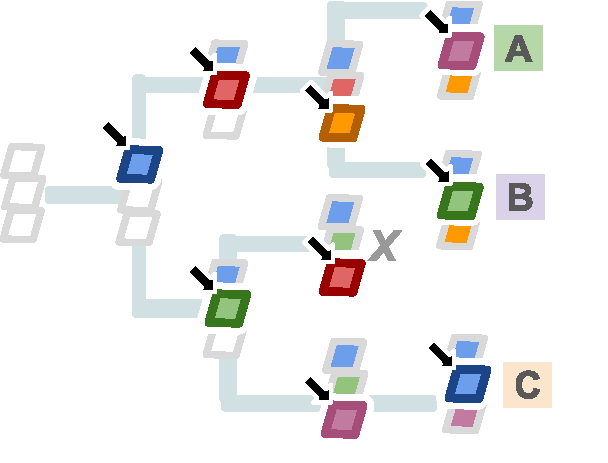
\includegraphics[height=1.1in]{img/hstratschematic-evolve}
\subcaption{evolve}
\label{fig:hstratschematic:evolve}
\end{minipage}%
\vrule
\centering
\begin{minipage}{0.18\linewidth}
~

\includegraphics[height=1.1in]{img/hstratschematic-sample}
\subcaption{sample}
\label{fig:hstratschematic:sample}
\end{minipage}%
\vrule
\begin{minipage}{0.41\linewidth}
\centering
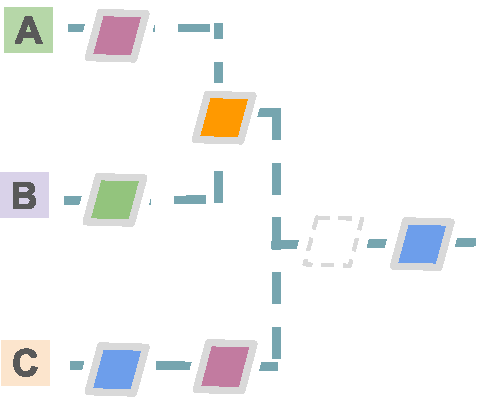
\includegraphics[height=1.1in]{img/hstratschematic-reconstruct}
\subcaption{reconstruct}
\label{fig:hstratschematic:reconstruct}
\end{minipage}
\end{minipage}%
~~
\begin{minipage}{0.43\textwidth}
\caption{%
\textbf{Overview of hereditary stratigraphy.}
\small
At runtime, genomes are annotated with randomly-generated heritable markers (panel \ref{fig:hstratschematic:evolve}).
To maintain fixed-memory footprint, some markers are overwritten.
Genomes of interest are sampled at runtime and from end state (panel \ref{fig:hstratschematic:sample}).
Decoded genome markers enable estimation of evolutionary relatedness (panel \ref{fig:hstratschematic:reconstruct}), subject to error from marker-value collisions and discarded markers.
Adapted from \citet{singhvi2025scalable}.
}
\label{fig:hstratschematic}
\end{minipage}
\end{figure*}


Under controlled conditions, such as laboratory experiments or evolution simulations, genetic material may be engineered to facilitate the accuracy and efficiency of estimating phylogenetic relatedness \citep{li2024reconstructing,ackley2023robust}.%
\footnote{Notably, Ackley has applied barcoding approaches to track recent ancestry among emergent replicators in a distributed fabric-computing context.}
Work developing hereditary stratigraphy (``hstrat'') methods seeks to operate analogously, providing techniques to organize genetic material in digital organisms that maximize reconstruction quality while minimizing memory footprint \citep{moreno2022hereditary}.
Hereditary stratigraphy components can be bundled with agent genomes in a manner akin to non-coding DNA (i.e., neutral with respect to agent traits and fitness), enabling generalizability across a wide variety of agent models.

Hereditary stratigraphy associates each generation along each lineage with an identifying ``fingerprint'' marker, referred to as a differentia.
On birth, each offspring receives a new differentia value and appends it to an inherited chronological record of past values --- corresponding to earlier generations along its lineage.
Under this scheme, mismatching differentia can be used to delimit the end of common ancestry between two organisms.
Figure \ref{fig:hstratschematic} summarizes this approach.

To save space, differentiae may be pruned away --- although, at the cost of reducing precision in inferring relatedness.
Using fewer bits per differentia can also provide many-fold memory savings; single bits or single bytes are appropriate for most use cases.

While inferring relatedness from biological sequence data can be a highly challenging and computationally-intensive problem \citep{miller2010creating},
the structured marker data used in hereditary stratigraphy somewhat ameliorates this challenge by allowing phylogeny reconstruction to be approached as a trie-building problem of identifying common string prefixes \citep{delabriandais1959file,moreno2024analysis}.
However, the presence of missing data due to some differentia being dropped to save memory complicates matters.

In the context of trie-building, missing marker time points (possessed by only a subset of organisms) effectively act as ``wildcard'' characters in prefix matching operations.
Therefore, placing an organism on a trie requires evaluating diverging string paths beyond the wildcard to identify further matches.
Given the likelihood of differentia value collisions for small differentia sizes (e.g., 1 bit), identifying the best-matching path after a wildcard value can require looking ahead several consecutive markers.
Furthermore, where consecutive wildcard values are encountered, the number of possible paths that must be explored can grow exponentially.

Although previous work has investigated the quality of phylogenies constructed from hereditary stratigraphy data using trie-based approaches \citep{moreno2025testing}, the computational intensity of the naive wildcard-matching approach has limited the scale of phylogenetic reconstructions investigated and restricted experimental throughput for smaller reconstructions.
Given the objective of hereditary stratigraphy methodology to facilitate studying very large-scale digital evolution experiments, achieving reconstruction efficiency sufficient for large-scale phyloanalysis is critical to the overall utility of the methodology in enabling observable experiments.

In this work, we describe an algorithm for efficient trie reconstruction in the face of missing data, and explore its performance characteristics.
The following section introduces our proposed ``shortcut'' algorithm for the trie building approach explored in this paper.
We then detail methods and results for benchmark trials assessing empirical scaling behavior and performance on large-scale billion-genome workloads.

Most existing artificial life work uses centralized tracking to maintain an exact, complete record of phylogenetic history comprising all parent-offspring relationships that have existed over the course of a simulation \citep{ray1992evolution,bohm2017mabe,de2012deap,garwood2019revosim,godin2019apoget,dolson2024phylotrackpy}.
Typically, records of extinct lineages are pruned to prevent memory bloat \citep{moreno2024analysis}.
Although direct tracking is well suited to serial simulation or centralized controller-worker schemes, runtime communication overheads and sensitivity to data loss impede scaling to highly distributed systems --- particularly those with lean memory capacity like the Cerebras WSE \citep{moreno2024analysis}.
To overcome this limitation, we have developed reconstruction-based approaches to \textit{in silico} phylogenetic tracking \citep{moreno2022hereditary}.
These approaches require no centralized data collection during simulation runtime; instead, they use \textit{post hoc} comparisons among end-state agent genomes to deduce approximate phylogenetic history --- akin to how DNA-based analyses describe natural history.
Figure \ref{fig:runtime-posthoc-schematic} summarizes this reconstruction-based strategy.

Although analogous work with natural biosequences is notoriously challenging and data-intensive \citep{neyman1971molecular,lemmon2013high},
the recently-developed hereditary stratigraphy annotation architecture is explicitly designed for fast, accurate, and data-lean reconstruction.
% Work reported here uses just 96 bits of tracking information per agent genome.
Designed to attach on underlying replicators as a neutral annotation (akin to noncoding DNA), it is a general-purpose technique potentially applicable across diverse study domains \citep{liben2008tracing,cohen1987computer,friggeri2014rumor}.
In a stroke of convergent thinking, \citet{ackley2023robust} reports use of ``bar code'' annotations on his self-replicators to achieve a measure of coarse-grained lineage tracing.

Since it was proposed, experimental work using hereditary stratigraphy has demonstrated viability in extracting information about underlying evolutionary conditions \citep{moreno2024ecology}, even at population scales reaching millions of agents/millions of generations using the 850,000 core Cerebras Wafer-Scale Engine hardware accelerator \citep{moreno2024trackable}.

\subsection{Outline}

collect, organize, assemble a comprehensive description of this methodology, reporting how reconstruction quality differs by configuration and underlying phylogenetic structure, explain and benchmark post-hoc inference for tree building, and demonstrate three on-hardware use cases on the Cerebras Wafer-Scale Engine.

A number of options exist in configuring hereditary stratigraphy algorithms, but no work has yet systematically investigated how they relate to quality of phylogenetic reconstruction.
In particular, it remains to be established how best to configure hereditary stratigraphy methodology to support use cases varying in scale, memory availability for annotation, and underlying evolutionary conditions.
In this work, we report annotate-and-reconstruct experiments that evaluate reconstruction quality under possible hereditary stratigraphy configurations across a variety of use cases.
We synthesize results from these experiments to suggest a prescriptive system of best practices for work with hereditary stratigraphy.
Analysis covers three primary configurable aspects of hereditary stratigraphy: (1) data structure implementation, (2) temporal data retention policy, and (3) size of stochastic lineage fingerprints.
This work, in conjunction with availability of open-source software library utilities for hereditary stratigraphy \citep{moreno2022hstrat}, is hoped to catalyze means for phylogenetic analysis across a range of large-scale digital evolution projects.

In this paper, we report new software and algorithms that harness the Cerebras Wafer-Scale Engine to enable radically scaled-up agent-based evolution while retaining key aspects of observability necessary to support hypothesis-driven computational experiments.
Implementation comprises two primary aspects:
\begin{enumerate}
  \item an asynchronous island-based genetic algorithm (GA) suited to the memory-scarce, highly-distributed, data-oriented WSE architecture, and
  \item a fundamental reformulation of hereditary stratigraphy's core storage and update procedures to achieve fast, simple, resource-lean annotations compatible with unconventional, resource-constrained accelerator and embedded hardware like the WSE.
\end{enumerate}

Both are implemented in Cerebras Software Language (CSL) and validated using Cerebras' SDK hardware emulator.
We use benchmark experiments to evaluate the runtime performance characteristics of the new hereditary stratigraphy algorithms in isolation and in the integrated context providing tracking-enabled support for the island-model GA.
In conjunction, we report emulated and on-device trials that validate phylogenetic reconstructions and demonstrate their suitability for inference of underlying evolutionary conditions.

Results from both experiments are promising.
We find that new surface-based algorithms greatly improve runtime performance.
Scaled-down emulator benchmarks and early on-hardware trials indicate potential for simple agent models --- with phylogenetic tracking enabled --- to achieve on the order of quadrillions of agent replication events a day at full wafer scale, with support for population sizes potentially reaching hundreds of millions.
Further, using proposed techniques, phylogenetic analyses of simulations spanning hundreds of thousands of PEs succeed in detecting differences in adaptive dynamics between alternate simulation conditions.

\subsection{introduction outline}

\begin{itemize}
\item blurb about AI/ML accelerators (steal from current surface draft?)
\item explain importance of phylogeny data
\item blurb about reconstruction vs. tracking (Figure \ref{fig:tracking-vs-reconstruction-schematic})
    \begin{itemize}
    \item note CRISPR/barcode-based approaches used in experimental biology
    \item note reconstruction quality trade-off (Figure \ref{fig:colorclade})
    \item emphasize that direct tracking is the most common choice for existing serial applications
    \end{itemize}
\item blurb about difficulty tracking phylogenies in highly-distributed settings
   \begin{itemize}
   \item extinction tracking (cite arxiv/phylotrackpy)
   \item memory use in distributed settings (Figure \ref{fig:msprime-memory-estimate})
   \item note about implementation simplicity
      \begin{itemize}
      \item although not a major issue from a theoretical angle, in practice implementation complexity is a major issue from a practical angle (especially given the vendor-/hardware-specific programming languages among emerging accelerators)
      \item predictable memory use (comptime-known, non-dynamic memory)
      \item communication patterns/routes (no additional PE-to-PE or host-sevice communication beyond migration)
      \end{itemize}
   \item data loss/node failure; indefinite scalability
   \end{itemize}
\item burb about broader topic of statistical observability (borrow from EXPRESS grant)
\item tie to OEE (alife) and to multiscale modeling (complex systems/evolutionary biology)
\item outline paper results and contribution
   \begin{itemize}
   \item introducing novel approach for distributed tracking in HPC, inspired by
   \item introducing efficient algorithms for marker layout and reconstruction
   \item providing evidence-based guidelines for effective use (steady vs. tilted vs. hybrid, num bits in column, fossils)
   \item item motivating use with examples on next-generation hardeare (e.g., WSE)
   \item broader paradigm of best-effort/statistical observability in HPC --- using statistics from working with physical systems)
   \end{itemize}
\end{itemize}

\subsection{methods outline}

\begin{itemize}
\item technical details of hereditary stratigraphy \citep{moreno2024algorithms}; briefly note history (columns, as originally proposed in \citep{moreno2022hereditary})
\item reconstruction algorithm overview (Figure \ref{fig:algorithm-diagram}, Algorithm \ref{fig:consolidation}); briefly note history (distance-based approaches in \citep{moreno2022hereditary}, naive algorithm in \citep{moreno2023toward})
\item msprime methods used to create estimates in Figure \ref{fig:msprime-memory-estimate}
\item transplant experiment setup from \citep{moreno2025testing}, will need to describe new fossil quality trials
\item transplant benchmark setup from \citep{singhvi2025scalable}
\item configurations for various WSE-2 and WSE-3 demonstrations
\item open-source software acknowledgement (incl \citep{zanini2025unified})
\item supplement: overview of where to find different parts of code (because spread across projects)
\end{itemize}

\subsection{results outline}

\begin{itemize}
\item reconstruction quality
   \begin{itemize}
   \item steady vs. tilted vs. hybrid results (\Cref{fig:steady-vs-tilted-summary,fig:recency-structure} \citep{moreno2025testing})
   \item TODO new fossil reconstruction quality results (Vivaan)
   \end{itemize}
\item reconstruction algorithm
   \begin{itemize}
  \item scaling behavior (\Cref{fig:asymptotic,fig:scaling} \citep{singhvi2025scalable})
   \item billion tip reconstruction profile (Figure \ref{fig:billion-tip-time} \citep{singhvi2025scalable})
   \item TODO (supplement) new reconstruction quality comparisons vs. naive (Vivaan)
   \end{itemize}
\item demonstrations
  \begin{enumerate}
  \item on-device cost benchmark from \citep{moreno2024trackable}
  \item phylogeny topology: purifying vs. adaptive (Figure \ref{fig:on-device}) \citep{moreno2024trackable}
  \item phylogeny trait distribution: preliminary WSE MLS results (Figure \ref{fig:use-case-mls} \citep{moreno2025extending})
  \item cellular automata (WSE3 demo, Figure \ref{fig:use-case-gol}, cite cliff?)
  \end{enumerate}
\end{itemize}

\subsection{conclusion outline}

\begin{itemize}
\item note overlap with exact tracking via imaging in e.g., E coli
\item what do you do with a billion tip phylogeny?
   \begin{itemize}
   \item pipeline builds trees efficiently enough that analysis and visualization become the bottleneck
   \item broader emerging problem --- e.g., very large reconstructions from CRISPR barcoding paper
   \item transplant software ecosystem blurb from \citep{singhvi2025scalable}
   \end{itemize}
\end{itemize}

\subsection{Introduction Figures}

\FloatBarrier

% graphic source: https://docs.google.com/presentation/d/11NBuIXM8JQMI2pnPQOirfBzwYOAdVX4sol6ymvlcvqA
\begin{figure}
\begin{minipage}{0.65\linewidth}
\begin{subfigure}{0.55\linewidth}
  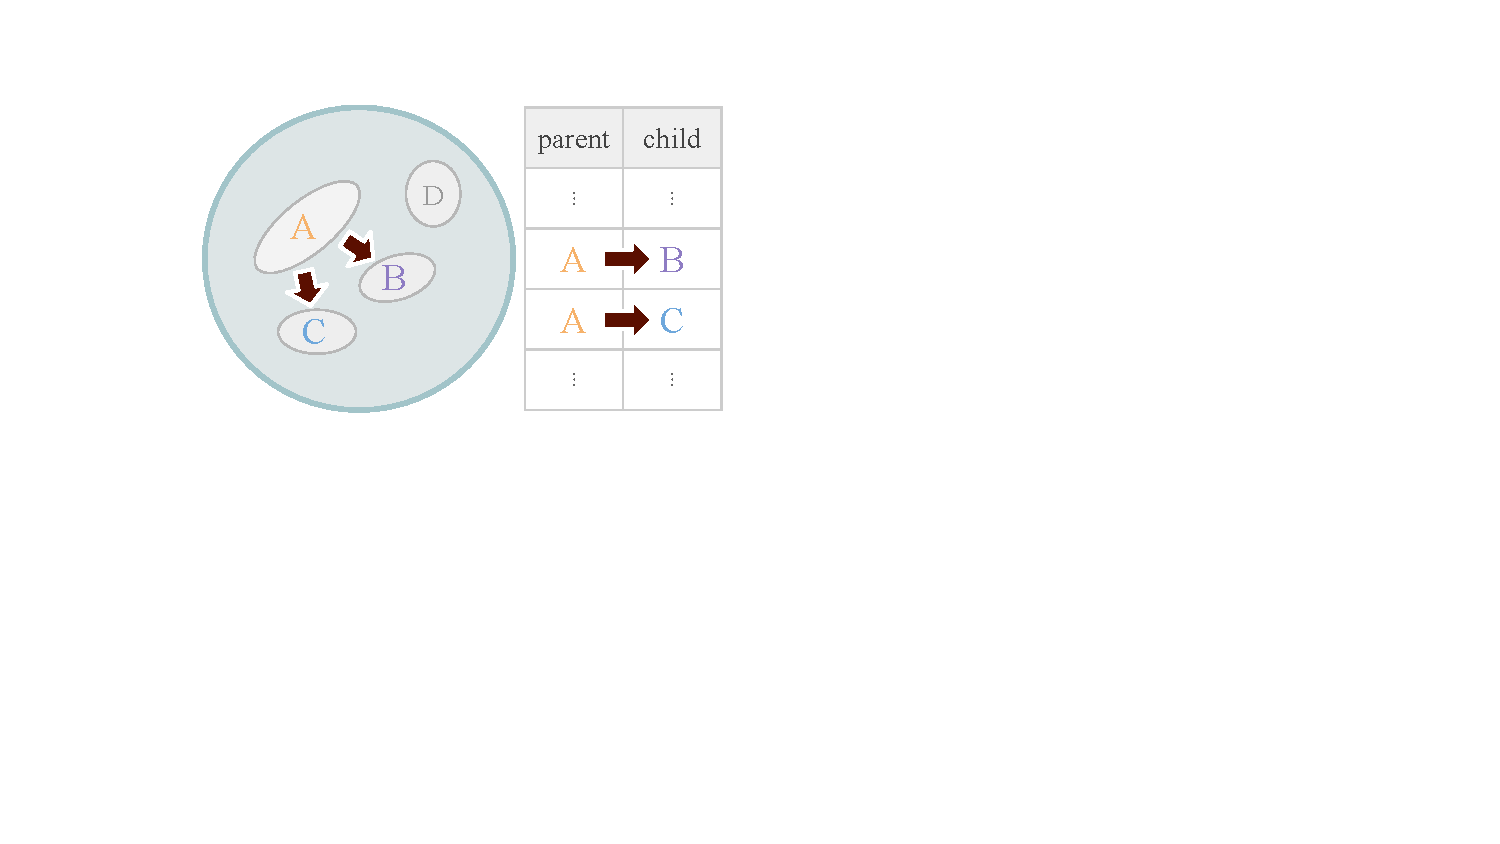
\includegraphics[width=\linewidth]{img/tracking-schematic}
  \caption{\footnotesize tracking approach}
  \label{fig:tracking-vs-reconstruction-schematic:tracking}
\end{subfigure}%
\begin{subfigure}{0.025\linewidth}~\end{subfigure}%
\vrule
\begin{subfigure}{0.025\linewidth}~\end{subfigure}%
\begin{subfigure}{0.35\linewidth}
  \centering
  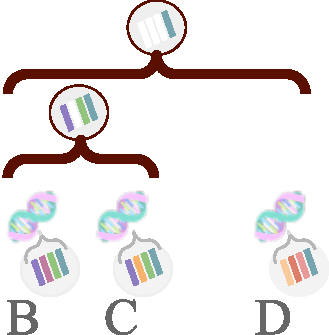
\includegraphics[width=\linewidth]{img/reconstruction-schematic}
  \caption{\footnotesize reconstruction approach}
  \label{fig:tracking-vs-reconstruction-schematic:reconstruction}
\end{subfigure}%
\begin{subfigure}{0.02\linewidth}~\end{subfigure}%
\end{minipage}%
\begin{minipage}{0.35\textwidth}
  \caption{%
  \textbf{Phylogeny tracking versus reconstruction.}
  \footnotesize
  TODO.
  }
  \label{fig:tracking-vs-reconstruction-schematic}
\end{minipage}
\end{figure}


% graphic source https://docs.google.com/presentation/d/10IDom7LfeptDY-rK8ClatmKTfRuEoFrzMhTkaZrDVIA
\begin{figure*}[h]

\centering
\begin{minipage}{0.55\textwidth}

\begin{minipage}{0.41\linewidth}
\centering
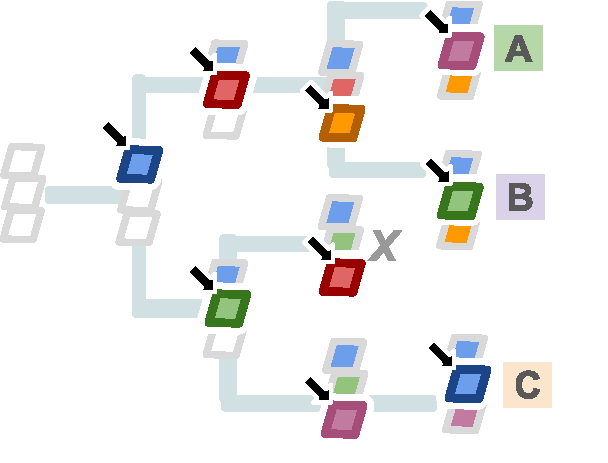
\includegraphics[height=1.1in]{img/hstratschematic-evolve}
\subcaption{evolve}
\label{fig:hstratschematic:evolve}
\end{minipage}%
\vrule
\centering
\begin{minipage}{0.18\linewidth}
~

\includegraphics[height=1.1in]{img/hstratschematic-sample}
\subcaption{sample}
\label{fig:hstratschematic:sample}
\end{minipage}%
\vrule
\begin{minipage}{0.41\linewidth}
\centering
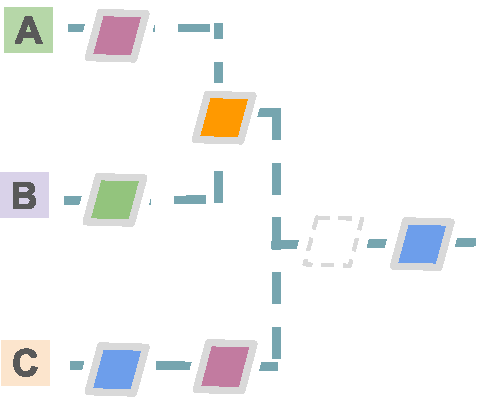
\includegraphics[height=1.1in]{img/hstratschematic-reconstruct}
\subcaption{reconstruct}
\label{fig:hstratschematic:reconstruct}
\end{minipage}
\end{minipage}%
~~
\begin{minipage}{0.43\textwidth}
\caption{%
\textbf{Overview of hereditary stratigraphy.}
\small
At runtime, genomes are annotated with randomly-generated heritable markers (panel \ref{fig:hstratschematic:evolve}).
To maintain fixed-memory footprint, some markers are overwritten.
Genomes of interest are sampled at runtime and from end state (panel \ref{fig:hstratschematic:sample}).
Decoded genome markers enable estimation of evolutionary relatedness (panel \ref{fig:hstratschematic:reconstruct}), subject to error from marker-value collisions and discarded markers.
Adapted from \citet{singhvi2025scalable}.
}
\label{fig:hstratschematic}
\end{minipage}
\end{figure*}


\begin{figure}[h]
\centering
\begin{minipage}{0.62\linewidth}
    \centering
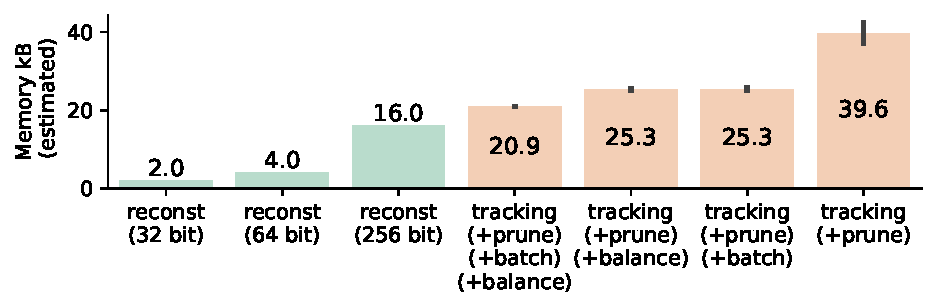
\includegraphics[width=0.95\linewidth]{binder/binder-2025-10-28-trafficsim_msprime.ipynb/binder/teeplots/2025-10-28-trafficsim_msprime/hue=flavor+viz=barplot+x=strategy+y=memory-use-kb+ext=.pdf}
\end{minipage}%
\begin{minipage}{0.38\linewidth}
\caption{%
\textbf{Per-node memory use for phylogeny tracking techniques.}
\footnotesize
Memory estimates for tracking approaches are estimated according to coalescent trees sampled using msprime, to simulate phylogeny migration dynamics across a processor grid.
We assume extinct lineages to be removed from memory through extinction tracking --- meaning that exact records need only be stored for extant lineages (pruning).
We assume unifurcations within the scope of a single PE are collapsed.
For batching optimization, it is assumed that the simulation is halted every 100,000 generations for a clean-up phase where data is offloaded off the chip to free on-chip memory from elapsed history.
For balancing optimization, it is assumed that memory load is shared evenly across the chip so that data capacity is necessary just on behalf of average behavior, not necessarily the most extreme cases requiring a buffer leeway.
Serial direct tracking represents a lower bound on memory usage for a bifurcating phylogeny, which scales as $2B$ population size.
A population size of 512 agents per node is assumed, with demes arranged in a 2D grid and agents migrating between neighboring demes at a rate of 5\%.
Further details on estimation methodology is provided in Section \ref{sec:TODO}.
}
\label{fig:msprime-memory-estimate}
\end{minipage}
\end{figure}


\begin{figure}[h]
\begin{minipage}{0.33\linewidth}
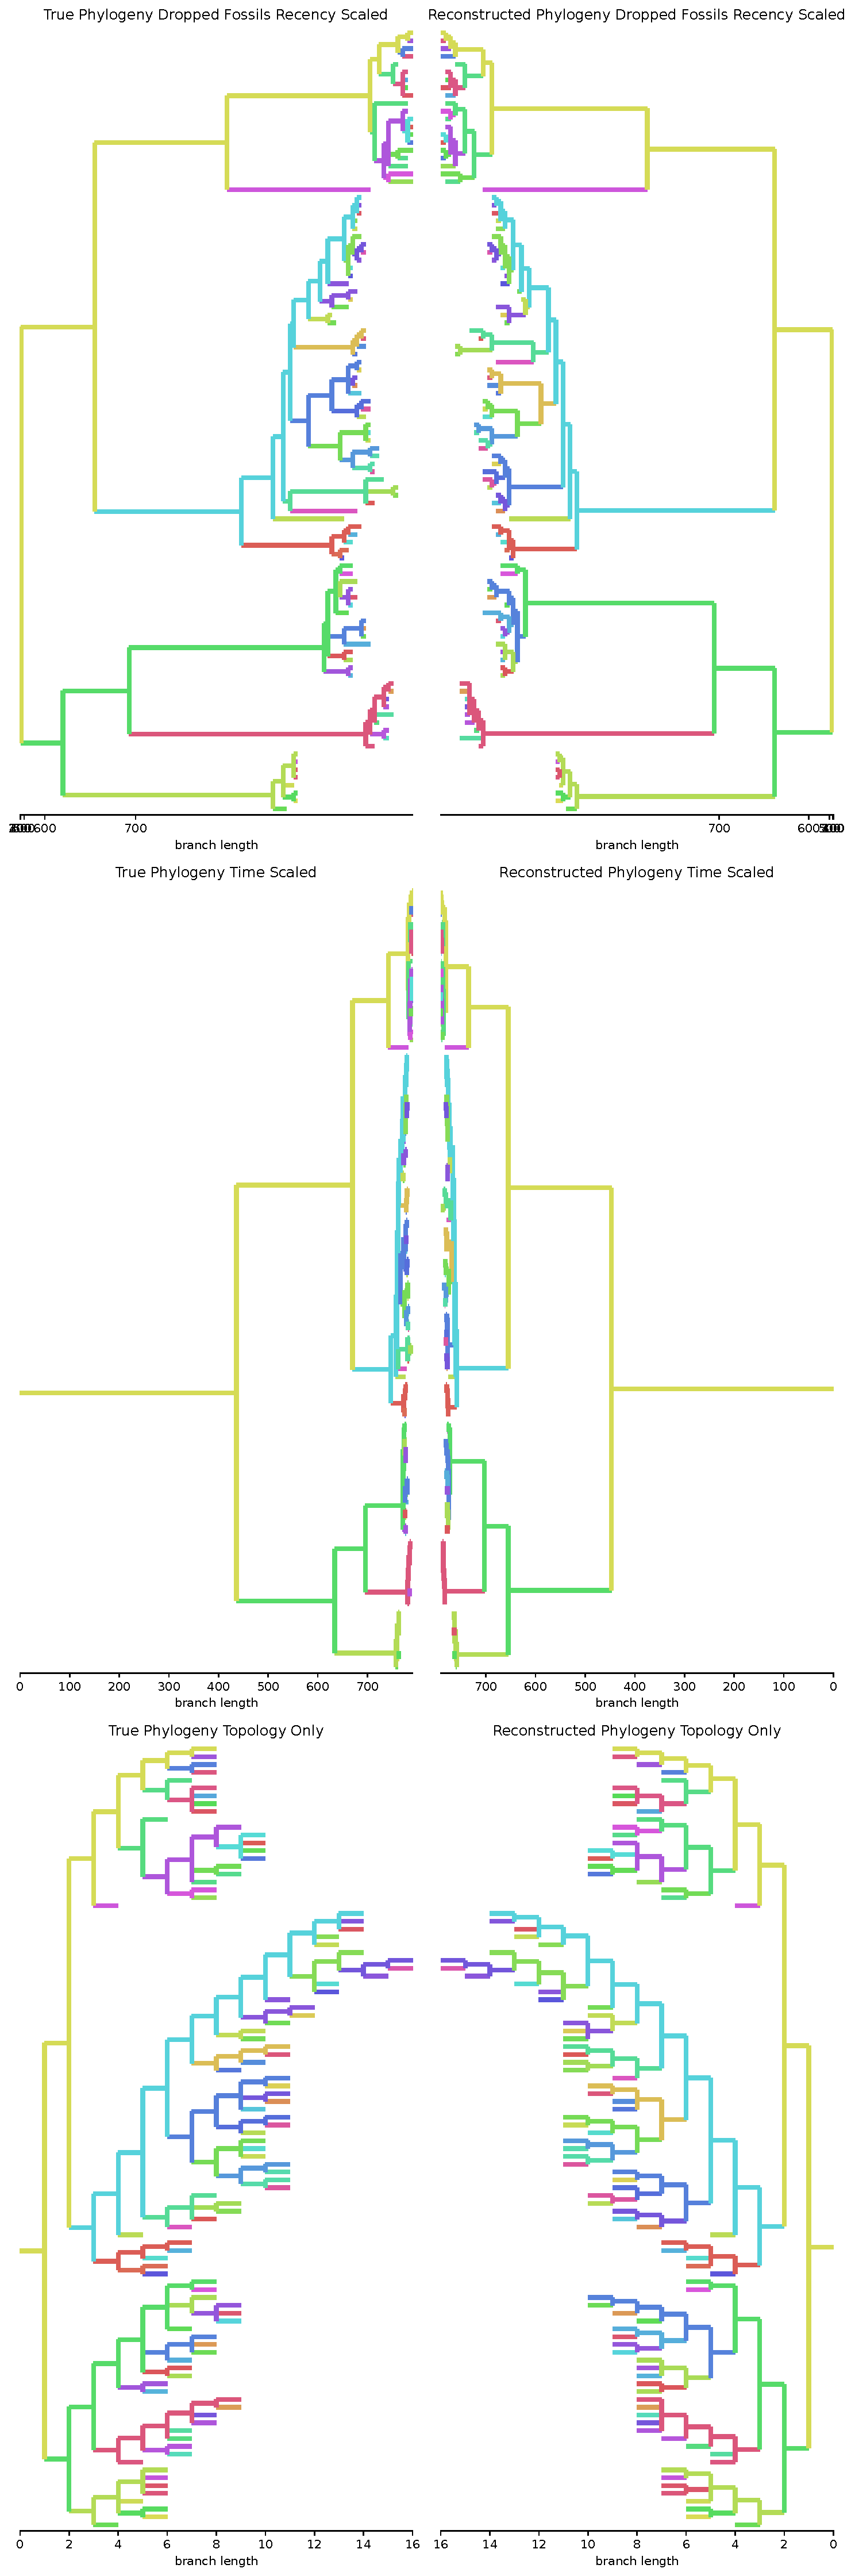
\includegraphics[width=\columnwidth,trim={0 52cm 0 0.8cm},clip]{img/colorclade.pdf}
\end{minipage}%
\begin{minipage}{0.33\linewidth}
\caption{\textbf{Sample comparison of true and reconstructed phylogenies.}
\footnotesize
Generated using a tilted retention policy and a surface of 32 bits. The true phylogeny is on the left and the reconstructed phylogeny is on the right.
Colors are based on a hash from the taxon label for each tip to better facilitate visual comparison. Reconstruction error for this reconstruction was 2.6\%. Visualization created with colorclade \citep{moreno2024colorclade}.
}
\label{fig:colorclade}
\end{minipage}
\end{figure}


\section{Introduction} \label{sec:introduction}

Key aspects of the study of evolution, whether biological or digital, revolve around understanding the flow of genetic material among large populations of organisms.
As such, phylogenetic analyses assessing ancestry trees representing organisms' evolutionary histories are a core tool in evolutionary biology.

In biology, phylogeny estimations are typically reconstructed through \textit{post hoc} analysis of genetic similarities among organisms.
In contrast, direct, exact tracking at runtime is typical in \textit{in silico} experiments.
However, in memory-constrained parallel and distributed computing contexts, \textit{post hoc} reconstruction approaches can become advantageous owing to runtime synchronization and storage costs of direct tracking.

Akin to biological studies, efficacy of phylogenetic analysis in such digital experiments hinges on fast, accurate methods to estimate ancestry trees from genome data.
In this work, we present a novel trie-building algorithm that greatly reduces compute time necessary to reconstruct phylogenies from special-purpose markers on digital genomes, while producing results equivalent to a naive approach.

\subsection{Applications of Phylogenetic Analysis}

% \subsection{Reconstructing Biological Phylogenies} \label{sec:introduction:bioreconst}

% In biological studies, phylogenetic reconstruction methods typically work by assessing nucleotide changes between aligned DNA sequences from sample organisms.
% Approaches include distance-based methods, where a distance matrix between organisms is computed and processed with methods such as neighbor-joining \citep{saitou1987neighbor}; or character-based methods, such as maximum-parsimony \citep{sober1991reconstructing}, which seeks to minimize the number of evolutionary changes necessary to explain an evolutionary history --- and maximum-likelihood \citep{felsenstein1981evolutionary}, which infers tree topologies maximizing a likelihood function \citep{de2014phylogenetic}.

\subsection{Phylogenies and Digital Evolution} \label{sec:introduction:digital}


Given the programmatic observability of digital simulations, digital evolution platforms typically incorporate direct tracking methods that record lineage ancestry as the simulation runs.
General-purpose phylogeny-tracking libraries exist for this purpose \citep{dolson2024phylotrack}, although many platforms simply incorporate bespoke implementations into their own software \citep{ofria2004avida}.

\subsection{Scaling Up Digital Evolution Experiments} \label{sec:introduction:distributed}

To achieve large-scale digital evolution experiments, it is necessary to move from a single-processor system to a more distributed approach with many computing units \citep{moreno2024trackable}.
In large-scale, many-processor simulations, however, challenges arise in managing a comprehensive record of ancestry.
To control memory use, it is typically necessary to trim away records of extinct lineages when performing direct tracking.
Detecting extinctions, however, introduces implementation complexity and overhead costs when lineage histories span across multiple processors.
Exhaustive tracking is also sensitive to data loss from crashed hardware or dropped messages, which has been highlighted as a key consideration in achieving very large-scale artificial life systems \citep{ackley2016indefinite,ackley2014indefinitely}.

Challenges associated with comprehensive tracking are especially acute in specialized hardware accelerator devices, which represent a promising emerging direction in high-performance computing \citep{emani2024democratizing}.
In incorporating thousands of processor cores per device, these hardware architectures impose trade-offs in memory capacity limitations and data locality restrictions that limit the feasibility of comprehensive tracking.
In such contexts, reconstruction-based approaches can provide an attractive balance between data fidelity and data collection overhead.

\subsection{Hereditary Stratigraphy} \label{sec:introduction:hstrat}



\section{Introduction} \label{sec:introduction}


\section{Introduction}

% defining? fundamental?
A quintessential characteristic of computational artificial life experiments is the near total malleability of the simulacrum \citep{pattee1989simulations}.
Indeed, exploration of arbitrary possibilities `as they could be' is the core of artificial life's role as a tool for inquiry \citep{langton1997artificial}.
Such near-limitless freedom to realize arbitrary system configurations, however, can obscure an intrinsic limitation of most computational artificial life work: scale.

Take, for instance, the Avida platform, which instantiates populations of self-replicating computer programs for evolution experiments.
When running on a single CPU, this system can support about 20,000 generations per day, or about two hundred million individual replication cycles daily \citep{ofria2009artificial}.
By way of comparison, \textit{E. coli} populations within individual flasks of the Lenski Long-Term Evolution Experiment undergo only six doublings per day, meaning their generations take orders of magnitude longer than Avidians \citep{good2017dynamics}.
(In continuous culture, though, the rate can be c. 72 generations per day.)
Indeed, such capability for fast generational turnover has been a key motivation for using artificial life systems to study evolution.
However, the effective population size of flasks in the Long-Term Evolution Experiment is orders of magnitude larger than Avida's population size: 30 million vs. 10,000.
Consequently, these systems actually exhibit a similar number of replication events per day.
This pattern of dramatically faster generation times than those observed in nature and dramatically smaller populations largely generalizes across artificial life systems.
%Although ALife systems can typically observe generational cycles at orders-of-magnitude faster rates than their biological counterparts, population sizes are often limited and,
Of course, any such comparisons should also note profound discrepancies between the genetic, phenotypic, and environmental richness of biological organisms and ALife models.

% Adversely? Crucially? Conversely? Formidably? Aversely? Cumbrously?

\subsection{Untapped Emerging Hardware}

In retrospect, connectionist artificial intelligence turns out to have been profoundly scale-dependent.
The utility and ubiquity of ANNs have exploded in tandem with torrential growth in training set sizes, parameter counts, and training FLOPs \citep{marcus2018deep}.
Recruitment of multi-GPU training for image classification, requisite particular accommodating adjustments to the underlying deep learning architecture, is commonly identified as the watershed moment to this transformation
 \citep{krizhevsky2012imagenet}.
Commercial investment in AI capabilities then set in motion a virtuous cycle of further-enabling hardware advances \citep{jouppi2017datacenter}.
Indeed, the scaling relationship between deep learning and training resources has itself become a major area of active study, with expectation for this virtuous cycle to continue through the foreseeable future \citep{kaplan2020scaling}.

A major upshot of the deep learning race is the emergence of spectacularly capable next-generation compute accelerators \citep{zhang2016cambricon,emani2021accelerating,jia2019dissecting,medina2020habana}.
Although tailored expressly to deep learning workloads, these hardware platforms represent an exceptional opportunity to leapfrog progress on grand challenges in artificial life.
The emerging class of fabric-based accelerators, led by the 850,000 core Cerebras CS-2 Wafer-Scale Engine (WSE) \citep{lauterbach2021path,lie2022cerebras}, holds particular promise as a vehicle for artificial life models.
This architecture interfaces multitudinous processing elements (PEs) in a physical lattice, with PEs executing independently with private on-chip memory and interacting locally through a network-like interface.

In this work, we explore how such hardware might be recruited for large-scale digital evolution, demonstrating a genetic algorithm implementation tailored to the dataflow-oriented computing model of the CS-2 platform.
Indeed, rapid advances in the capability of accelerator devices, driven in particular by market demand for deep learning operations, are anticipated to drive advances in agent-based model capabilities \citep{perumalla2022computer}.
The upcoming CS-3 chip, for instance, supports clustering potentially thousands of constituent accelerators \citep{moore2024cerebras}.


\subsection{Maintaining Observability}

Orthogonalities between the fundamental structure and objectives of AI and artificial life methods will complicate any effort to requisition AI hardware for artificial life purposes.
In common use, deep learning operates as a black box medium \citep{loyola2019black} (but not always \citep{mahendran2015understanding}).
This paradigm de-emphasizes accessibility of inner state.
In contrast, artificial life more often functions as a tool for inquiry.
This goal emphasizes capability to observe and interpret underlying simulation state \citep{moreno2023toward,horgan1995complexity}.
(A similar argument holds for ALife work driven by artistic objectives, as well.)

Unfortunately, scale complicates simulation observability.
It is not uncommon for the volume and velocity of data streams from contemporary simulation to outstrip hardware bandwidth and storage capacity \citep{osti_1770192}.
Extensive engineering effort will be required to ensure large-scale simulation retains utility in pursuing rigorous hypothesis-driven objectives.

Here, we confront just a single aspect of simulation observability within distributed evolutionary simulation: phylogenetic history (i.e., evolutionary ancestry relationships).
Phylogenetic history plays a critical role in many evolution studies, across study domains and \textit{in vivo} and \textit{in silico} model systems alike \citep{faithConservationEvaluationPhylogenetic1992,STAMATAKIS2005phylogenetics,frenchHostPhylogenyShapes2023,kim2006discovery,lewinsohnStatedependentEvolutionaryModels2023a,lenski2003evolutionary,moreno2021case}.
Phylogenetic analysis can trace the history of notable evolutionary events (e.g., extinctions, evolutionary innovations), but also characterize more general questions about the underlying mode and tempo of evolution \citep{moreno2023toward,hernandez2022can,shahbandegan2022untangling,lewinsohnStatedependentEvolutionaryModels2023a}.
Particularly notable, recent work has used comparison of observed phylogenies against those produced under differing simulation conditions to test hypotheses describing underlying dynamics within real-life evo-epidemiological systems \citep{giardina2017inference,voznica2022deep}.
Additionally, \textit{in silico}, phylogenetic information can even serve as a mechanism to guide evolution in application-oriented domains \citep{lalejini2024phylogeny,lalejini2024runtime,murphy2008simple,burke2003increased}.

\subsection{Decentralized Phylogenetic Tracking}

% graphic source: https://docs.google.com/presentation/d/11NBuIXM8JQMI2pnPQOirfBzwYOAdVX4sol6ymvlcvqA
\begin{figure}
\begin{minipage}{0.65\linewidth}
\begin{subfigure}{0.55\linewidth}
  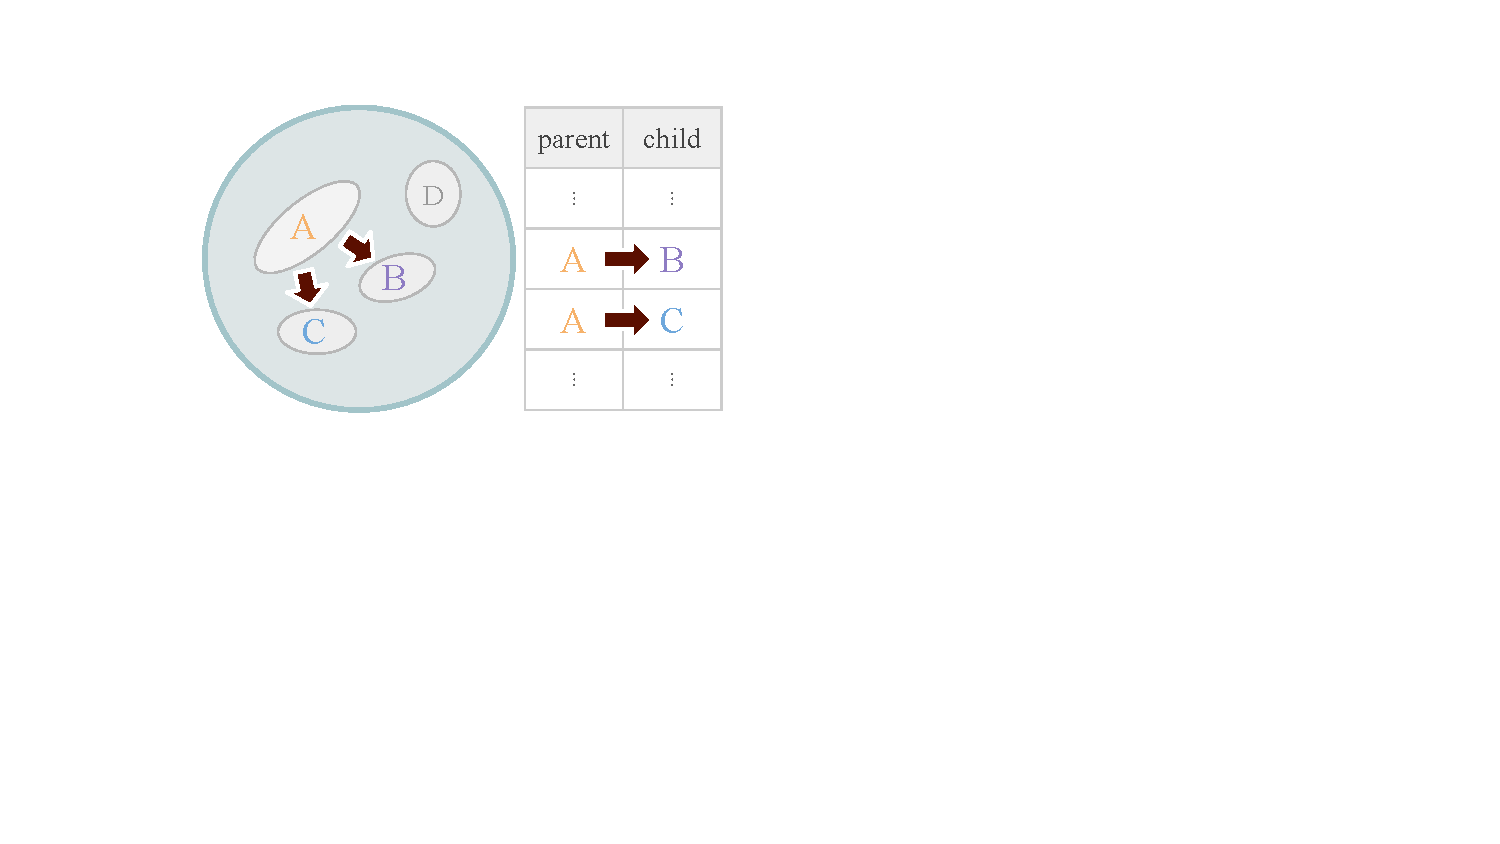
\includegraphics[width=\linewidth]{img/tracking-schematic}
  \caption{\footnotesize tracking approach}
  \label{fig:tracking-vs-reconstruction-schematic:tracking}
\end{subfigure}%
\begin{subfigure}{0.025\linewidth}~\end{subfigure}%
\vrule
\begin{subfigure}{0.025\linewidth}~\end{subfigure}%
\begin{subfigure}{0.35\linewidth}
  \centering
  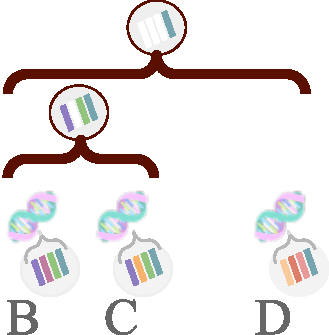
\includegraphics[width=\linewidth]{img/reconstruction-schematic}
  \caption{\footnotesize reconstruction approach}
  \label{fig:tracking-vs-reconstruction-schematic:reconstruction}
\end{subfigure}%
\begin{subfigure}{0.02\linewidth}~\end{subfigure}%
\end{minipage}%
\begin{minipage}{0.35\textwidth}
  \caption{%
  \textbf{Phylogeny tracking versus reconstruction.}
  \footnotesize
  TODO.
  }
  \label{fig:tracking-vs-reconstruction-schematic}
\end{minipage}
\end{figure}

